\documentclass[aps, prl, twocolumn, superscriptaddress, final]{revtex4}
\pdfoutput=1


\usepackage[utf8]{inputenc}
\usepackage[T1]{fontenc}
\usepackage{amsmath}
\usepackage{amssymb}
\usepackage{float}
\usepackage{graphicx}
\usepackage{microtype}
\usepackage{tikz}


\newcommand{\abs}[1]{\left| #1 \right|}
\DeclareMathOperator{\sech}{sech}

\newcommand*\circled[1]{
  \tikz[baseline=(char.base)]{
    \node[shape=circle,draw,inner sep=0.5pt] (char) {#1};
  }
}


\begin{document}

\title{Cherenkov radiation and scattering of external dispersive waves by two-color solitons}

\author{Ivan Oreshnikov}
\email{oreshnikov.ivan@gmail.com}
\affiliation{Max Planck Institute for Intelligent Systems, Max-Planck-Ring 4, 72076 T\"ubingen, Germany}

\author{Oliver Melchert}
\affiliation{Cluster of Exellence PhoenixD, Welfengarten 1, 30167 Hannover, Germany}
\affiliation{Institute of Quantum Optics, Leibniz Universit\"at Hannover, Welfengarten 1, 30167 Hannover, Germany}
\affiliation{Hannover Centre for Optical Technologies, Neinburger Strasse 17, 30167 Hannover, Germany}

\author{Stephanie Willms}
\affiliation{Cluster of Exellence PhoenixD, Welfengarten 1, 30167 Hannover, Germany}
\affiliation{Institute of Quantum Optics, Leibniz Universit\"at Hannover, Welfengarten 1, 30167 Hannover, Germany}

\author{Surajit Bose}
\affiliation{Institute of Quantum Optics, Leibniz Universit\"at Hannover, Welfengarten 1, 30167 Hannover, Germany}

\author{Ihar Babushkin}
\affiliation{Cluster of Exellence PhoenixD, Welfengarten 1, 30167 Hannover, Germany}
\affiliation{Institute of Quantum Optics, Leibniz Universit\"at Hannover, Welfengarten 1, 30167 Hannover, Germany}

\author{Ayhan Demircan}
\affiliation{Cluster of Exellence PhoenixD, Welfengarten 1, 30167 Hannover, Germany}
\affiliation{Institute of Quantum Optics, Leibniz Universit\"at Hannover, Welfengarten 1, 30167 Hannover, Germany}
\affiliation{Hannover Centre for Optical Technologies, Neinburger Strasse 17, 30167 Hannover, Germany}

\author{Alexey Yulin}
\affiliation{Department of Nanophotonics and Metamaterials, ITMO University, Kronverskiy pr. 49, 19701 St.~Petersburg, Russia}

\begin{abstract}
  In dispersion landscapes with two separate regions of anomalous dispersion it is possible to create a quasi-stable two-color solitary wave. In this paper we consider how those waves interact with dispersive radiation, including the processes of Cherenkov radiation generation as well as the processes of external wave scattering. We derive the analytic resonance conditions and verify them through numeric experiments.
\end{abstract}

\maketitle

\section{Introduction}

From the prior work~\cite{melchert2019soliton} we know that if the dispersion landscape $\beta(\omega)$ has two regions of anomalous dispersion separated by a region of normal dispersion, it is possible to create a quasi-stable configuration of two tightly-coupled solitons each propagating on its own carrier frequency. This coupled state, especially in the process of initial evolution, sheds dispersive waves that resembles Cherenkov radiation that is observed for other types of solitary waves in vast variety of settings~\cite{akhmediev1995cherenkov, afanasjev1996effect, driben2015resonant, conforti2015parametric, wright2015ultrabroadband, oreshnikov2017dispersive}.

{
  % This is just a dummy text to see whether the general layout of the paper makes sense.
  \it
Nullam eu ante vel est convallis dignissim.  Fusce suscipit, wisi nec facilisis facilisis, est dui fermentum leo, quis tempor ligula erat quis odio.  Nunc porta vulputate tellus.  Nunc rutrum turpis sed pede.  Sed bibendum.  Aliquam posuere.  Nunc aliquet, augue nec adipiscing interdum, lacus tellus malesuada massa, quis varius mi purus non odio.  Pellentesque condimentum, magna ut suscipit hendrerit, ipsum augue ornare nulla, non luctus diam neque sit amet urna.  Curabitur vulputate vestibulum lorem.  Fusce sagittis, libero non molestie mollis, magna orci ultrices dolor, at vulputate neque nulla lacinia eros.  Sed id ligula quis est convallis tempor.  Curabitur lacinia pulvinar nibh.  Nam a sapien.

Pellentesque dapibus suscipit ligula.  Donec posuere augue in quam.  Etiam vel tortor sodales tellus ultricies commodo.  Suspendisse potenti.  Aenean in sem ac leo mollis blandit.  Donec neque quam, dignissim in, mollis nec, sagittis eu, wisi.  Phasellus lacus.  Etiam laoreet quam sed arcu.  Phasellus at dui in ligula mollis ultricies.  Integer placerat tristique nisl.  Praesent augue.  Fusce commodo.  Vestibulum convallis, lorem a tempus semper, dui dui euismod elit, vitae placerat urna tortor vitae lacus.  Nullam libero mauris, consequat quis, varius et, dictum id, arcu.  Mauris mollis tincidunt felis.  Aliquam feugiat tellus ut neque.  Nulla facilisis, risus a rhoncus fermentum, tellus tellus lacinia purus, et dictum nunc justo sit amet elit.
}

\section{Analytic model}%
\label{sec:AnalyticModel}

In this section we derive a perturbation theory that explains the resonance conditions that were proposed before, and then we extend to it to describe the process of external waves scattering on the soliton. We consider a non-envelope version of a nonlinear Schr\"odinger equation~\cite{amiranashvili2010hamiltonian}
\begin{equation}
  \label{eq:GNLSE}
  i \partial_{z} \tilde u
    + \beta(\omega) \tilde u(z, \omega)
    + \gamma(\omega) \mathcal{F} \left\{
      \abs{u}^{2} u(z, t)
    \right\}_{(\omega > 0)} = 0.
\end{equation}
Here and further tilde indicates a Fourier image of the field and $\mathcal{F}\left\{ \cdots \right\}_{(\omega > 0)}$ is the explicit Fourier transform over the positive frequencies.

\begin{widetext}

\noindent We start by introducing the ansatz that represents the solution as a sum of two single-frequency solitary waves $U_{1, 2}(z, t)$ and a residue radiation $\psi(z, t)$
\begin{gather}
  \label{eq:PerturbationAnsatz}
  u(z, t) = U_{1}(z, t) + U_{2}(z, t) + \psi(z, t) \\
  \abs{\psi} \ll \abs{U_{1}} \sim \abs{U_{2}}. \nonumber
\end{gather}
For the solitary waves $U_{1, 2}(z, t)$ we assume that they satisfy a pair of coupled nonlinear Schr\"odinger equations below
\begin{equation}
  \label{eq:CoupledSolitons}
  i \partial_{z} \tilde U_{n}
    + \beta_{n}(\omega) \tilde U_{n}(z, \omega)
    + \gamma(\omega) \mathcal{F} \left\{
      \abs{U_{n}}^{2} U_{n} + 2 \abs{U_{m}}^{2} U_{n}
    \right\}_{(\omega > 0)} = 0,
\end{equation}
where $n = 1, 2$ and $m = 2, 1 \ne n$. Essentially, this is an assumption that the solitons are coupled strictly by inducing a refractive-index potential on each other, and each soliton exists in some sort of a truncated dispersion landscape that is defined by the operator $\beta_{n}(\omega)$. A reasonable guess for a truncated operator is a parabolic approximation close to the carrier frequency
\begin{equation}
  \label{eq:TruncatedDispersionOperator}
  \beta_{n}(\omega) =
    \beta(\omega_{n}) +
    \beta'(\omega_{n}) (\omega - \omega_{n}) +
    \frac{1}{2} \, \beta''(\omega_{n}) (\omega - \omega_{n})^{2}
\end{equation}
We additionally propose that in the frame of reference of the individual soliton the envelope evolves with wavenumber $k_{n}(\omega)$ which we approximate by the wavenumber of the fundamental soliton in the ordinary nonlinear Schr\"odinger equation and a correction from a secondary soliton as
\begin{equation}
  \label{eq:SolitonWavenumber}
  k_{n}(\omega)
    \approx \frac{\gamma(\omega_{n}) A_{n}^{2}}{2}
    + \beta(\omega_{n}) + \beta'(\omega_{n}) (\omega - \omega_{n})
    + \gamma(\omega_{n}) A_{m}^{2}
\end{equation}
where $n = 1, 2$, $m = 2, 1 \ne n$ and $A_{n}$ is the soliton amplitude.

By substituting ansatz~\eqref{eq:PerturbationAnsatz} into equation~\eqref{eq:GNLSE}, linearizing with respect to perturbation $\psi(z, \omega)$ and discarding the terms corresponding to the soliton equations~\eqref{eq:CoupledSolitons} we get the equation for $\tilde \psi$
\begin{multline}
  \label{eq:PerturbationEquation}
  i \partial_{z} \tilde \psi
    + \beta(\omega) \tilde \psi(z, \omega)
    + \gamma(\omega) \mathcal{F}\left\{
      2 \abs{U_{1} + U_{2}}^{2} \psi +
      \left( U_{1} + U_{2} \right)^{2} \psi^{*}
    \right\}_{(\omega > 0)} = \\
    - \left[ \beta(\omega) - \beta_{1}(\omega) \right] \tilde U_{1}(z, \omega)
    - \left[ \beta(\omega) - \beta_{2}(\omega) \right] \tilde U_{2}(z, \omega)
    - \gamma(\omega) \mathcal{F} \left\{
      U_{2}^{2} U_{1}^{*} + U_{1}^{2} U_{2}^{*}
    \right\}_{(\omega > 0)}
\end{multline}
In the right-hand's side of equation~\eqref{eq:PerturbationEquation} we see two types of driving terms and each of those terms can be in resonance with the linear dispersive waves that exist in the system, if the particular wavenumber $k(\omega_{*})$ of the driving term is equal to a wavenumber of a dispersive wave $\beta(\omega)$ at some frequency $\omega_{*}$~\cite{akhmediev1995cherenkov, yulin2004four}. The first type of the terms is $\left[ \beta(\omega) - \beta_{n}(\omega) \right] U_{n}(z, \omega)$ which drives the generation of Cherenkov radiation by an individual soliton $U_{n}$ if the following resonance condition is satisfied
\begin{equation}
  \label{eq:CherenkovRadiationResonanceCondition}
  \beta(\omega) = k_{n}(\omega).
\end{equation}
The second type of the terms are $\gamma(\omega) \mathcal{F}\left\{ U_{2}^{2} U_{1}^{*} \right\}$ and $\gamma(\omega) \mathcal{F}\left\{ U_{1}^{2} U_{2}^{*} \right\}$ and they correspond to the process of four-wave mixing that in our case results in generation of dispersive radiation at some frequency where
\begin{equation}
  \label{eq:FWMRadiationResonanceCondition}
  \beta(\omega) = 2 k_{n}(\omega)  - k_{m}(\omega).
\end{equation}

Let us move on to the problem of external dispersive wave scattering. For that we split the perturbation into the incident and the scattered parts
\begin{equation}
  \label{eq:PerturbationSplit}
  \psi(z, t) = \psi_{\text{inc}}(z, t) + \psi_{\text{sc}}(z, t).
\end{equation}
We explicitly define $\psi_{\text{inc}}(z, t)$ as a linear wave that is propagating in a soliton-free medium
\begin{equation}
  \label{eq:IncidentFieldEquation}
  i \partial_{z} \tilde \psi_{\text{inc}}(z, t)
    + \beta(\omega) \tilde \psi_{\text{inc}}(z, t) = 0.
\end{equation}
Substituting equation~\eqref{eq:PerturbationSplit} into~\eqref{eq:PerturbationEquation} and eliminating the terms corresponding to~\eqref{eq:IncidentFieldEquation} we are left with equation for the scattered component
\begin{multline}
  \label{eq:ScatteredFieldEquation}
  i \partial_{z} \tilde \psi_{\text{sc}}
    + \beta(\omega) \tilde \psi_{\text{sc}}(z, \omega)
    + \gamma(\omega) \mathcal{F}\left\{
      2 \abs{U_{1} + U_{2}}^{2} \psi_{\text{sc}} +
      \left( U_{1} + U_{2} \right)^{2} \psi_{\text{sc}}^{*}
    \right\}_{(\omega > 0)} = \text{\ldots (omitted is the RHS from~\eqref{eq:PerturbationEquation})} \\
    - \gamma(\omega) \mathcal{F}\left\{
      2 \left(
        \abs{U_{1}}^{2} + U_{1} U_{2}^{*} + U_{2} U_{1}^{*} + \abs{U_{2}}^{2}
      \right) \psi_{\text{inc}} +
      \left(
        U_{1}^{2} + 2 \, U_{1} U_{2} + U_{2}^{2}
      \right) \psi_{\text{inc}}^{*}
    \right\}_{(\omega > 0)}
\end{multline}
\end{widetext}

In addition to the resonance terms already discussed in equation~\eqref{eq:PerturbationEquation} we see the terms that arise due to interaction between the incident radiation and the soliton. In here six new types of resonance behaviour are possible. The first one is due to terms $\abs{U_{1}}^{2} \psi_{\text{inc}}$ and $\abs{U_{2}}^{2} \psi_{\text{inc}}$, both with the resonance condition
\begin{equation}
  \label{eq:Type0ResonanceCondition}
  \beta(\omega_{\text{sc}}) = \beta(\omega_{\text{inc}})
\end{equation}
The next two are due to mixed terms $U_{1} U_{2}^{*} \psi_{\text{inc}}$ and $U_{2} U_{1}^{*} \psi_{\text{inc}}$, with the corresponding resonance condition being
\begin{equation}
  \label{eq:Type1ResonanceCondition}
  \beta(\omega_{\text{sc}}) = \pm k_{1} \mp k_{2} + \beta(\omega_{\text{inc}})
\end{equation}
Another two are due to $U_{n}^{2} \psi_{\text{inc}}^{*}$ and the resonance condition is
\begin{equation}
  \label{eq:Type2ResonanceCondition}
  \beta(\omega_{\text{sc}}) =
    2 k_{n}(\omega_{\text{sc}}) -
    \beta(\omega_{\text{inc}}), ~ n = 1, 2.
\end{equation}
The final one is due to $2 U_{1} U_{2} \psi_{\text{inc}}^{*}$ with the resonances at
\begin{equation}
  \label{eq:Type3ResonanceCondition}
  \beta(\omega_{\text{sc}}) =
    k_{1}(\omega_{\text{sc}}) +
    k_{2}(\omega_{\text{sc}}) -
    \beta(\omega_{\text{inc}}).
\end{equation}
To verify the predictions given by resonance conditions~\eqref{eq:CherenkovRadiationResonanceCondition},~\eqref{eq:FWMRadiationResonanceCondition},~\eqref{eq:Type0ResonanceCondition},~\eqref{eq:Type1ResonanceCondition},~\eqref{eq:Type2ResonanceCondition}, and~\eqref{eq:Type3ResonanceCondition} we proceed to numeric experiments.

\section{Numeric experiments}%
\label{sec:NumericExperiments}

To numerically integrate equation~\eqref{eq:GNLSE} we use the integrating factor method and transform the equation into a non-stiff version for a modified spectrum~\cite{dudley2010supercontinuum}. The modified equation can be handled by any standard ODE solver; we use a \texttt{scipy} interface to \texttt{ZVODE} solver from \texttt{ODEPACK}~\cite{hindmarsh1983odepack, virtanen2020scipy} (the complete set of sources codes used in the paper can be found in~\cite{sources}).

To study Cherenkov radiation of two color solitons we chain two separate simulations. First, following the prior work~\cite{melchert2019soliton}, we produce a two-color soliton by integrating an initial condition that is given by a sum of two fundamental solitons of standard NLSE
\begin{equation}
  \label{eq:SeedInitialCondition}
  u_{0}(t) =
      A_{1} \sech(t / T_{1}) e^{-i \omega_{1} t} +
      A_{2} \sech(t / T_{2}) e^{-i \omega_{2} t},
\end{equation}
where frequency $\omega_{1}$ is an arbitrary parameter (the only requirement is that it lies in the region of anomalous dispersion) and frequency $\omega_{2}$ is chosen such that group velocities of both the frequency components match
\begin{equation*}
  \beta'(\omega_{1}) = \beta'(\omega_{2}).
\end{equation*}
In most of the simulations in this paper we fix $T_{1} = T_{2} = 20$~fs and the amplitudes $A_{1}$ and $A_{2}$ are chosen as the fundamental soliton amplitudes at the corresponding frequencies. This configuration sheds significant amount of radiation and relaxes to a quasi-stable solitary wave. We take the output field of this seed simulation and suppress the radiation tails by multiplying it by a super-Gaussian window centered around the soliton peak. This isolated soliton serves as an input to the second simulation that is carried with the same parameters as the original one.

Once we suppress the initial radiation that is shed by the seed soliton during the relaxation process, the isolated soliton propagates generating a narrow-spectrum Cherenkov radiation. As an example we can consider Fig.~\ref{fig:Fig1}. Panel Fig.~\ref{fig:Fig1}b shows a normalized spectral density at the output of the simulation. There one can notice that on top of the input spectrum (plotted by thin black line) arise two additional spectral lines in the output spectrum (plotted by thicker gray line). Panel Fig.~\ref{fig:Fig2}c demonstrates resonance conditions~\eqref{eq:CherenkovRadiationResonanceCondition} and~\eqref{eq:FWMRadiationResonanceCondition}: black curve corresponds to the left-hand's side of both equations $\beta(\omega)$, horizontal lines correspond to the right-hand's sides. Intersections between the dispersive curve and the horizontal lines that contribute to Cherenkov radiation are marked separately: \circled{1}~is the radiation due to the second component of the soliton as predicted by equation~\eqref{eq:CherenkovRadiationResonanceCondition}, \circled{2}~is due to beat between the components with wavenumber $2 k_{2} - k_{1}$ as predicted by~\eqref{eq:FWMRadiationResonanceCondition}.

% A symmetric situation (resonances due to the second component and to beat with wavenumber $2 k_{1} - k_{2}$) turns out difficult to observe for the reasons yet unknown.

\begin{figure}[t]
  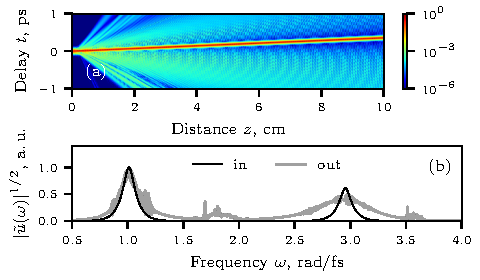
\includegraphics{{Figures/Fig1}.pdf}
  \caption{(color online) Cherenkov radiation of an isolated soliton produced by the simulation in Fig.~\ref{fig:Fig1}. (a) time-domain view (b) input and output spectra (c) resonance conditions diagram.}%
  \label{fig:Fig1}
\end{figure}

To study the scattering processes we perform the seed simulation and isolate the soliton as we did before. To that we add an incident dispersive wave in the form of a Gaussian pulse
\begin{equation*}
  \psi_{inc}(t) = A_{\text{inc}} \exp\left(
    - \frac{
      (t - t_{0})^{2}
    }{
      T_{\text{inc}}^{2}
    }
    - i \omega_{\text{inc}} t
  \right).
\end{equation*}
In this section we pick $A_{\text{inc}}$ as 1\% of the maximum amplitude of the isolated soliton and fix the width to 300~fs. Central location is chosen as $\pm1000$~fs from the soliton center (the sign depends on the relative group velocity between the soliton and the dispersive wave). In the process of evolution the incident radiation interacts with the soliton to produce the scattered radiation. This process can evolve in several different ways depending on the frequencies of the soliton and the incident radiation. In here we consider three concrete examples. In each of them the incident radiation is split between three different components.

The first configuration we consider is very close to the degenerate case where the wavenumbers of the individual soliton components $k_{1}$ and $k_{2}$ coincide. Equation~\eqref{eq:Type1ResonanceCondition} then turns into equation~\eqref{eq:Type0ResonanceCondition}. This case resembles the case of fundamental single-component solitons~\cite{yulin2004four}. However, due to shape of the dispersive curve $\beta(\omega)$ there is now more than one nontrivial solution to equation~\eqref{eq:Type0ResonanceCondition} and a single incident frequency corresponds up to four possible resonances. This configuration can be seen in Fig.~\ref{fig:Fig1}. In practice, only some of them actually contribute to the scattered radiation. Again, those solution are separately marked on a diagram on panel~\ref{fig:Fig1}c: \circled{$i$} corresponds both to the incident and the partially transmitted radiation, \circled{1} is the reflected component and \circled{2} is the additional transmitted component.

\begin{figure}[t]
  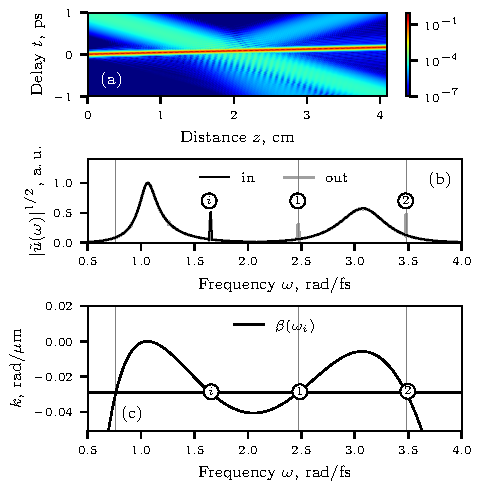
\includegraphics{{Figures/Fig2}.pdf}
  \caption{(color online) Scattering of a weak DW with carrier frequency $\omega_{\text{inc}} = 1.650$ on a soliton with first-component carrier frequency $\omega_{1} = 1.070$. (a) time-domain view (b) input and output spectra (c) resonance conditions diagram.}%
  \label{fig:Fig2}
\end{figure}

The second configuration (seen in Fig.~\ref{fig:Fig3}) is a case with significant difference between $k_{1}$ and $k_{2}$. Since~\eqref{eq:Type1ResonanceCondition} is no longer degenerate, the resonance diagram in Fig.~\ref{fig:Fig3}c is more complex. However, as one can notice, in that case only solution marked with \circled{2}, corresponding to the upper (i.e. ``$-, +$'') branch of~\eqref{eq:Type1ResonanceCondition}, contributes to the scattered radiation. Component \circled{1}, corresponding to the scattered radiation, comes from~\eqref{eq:Type0ResonanceCondition}. The unmarked spectral line close to $\omega \approx 2.4$ is the Cherenkov radiation of the soliton itself.

\begin{figure}[t]
  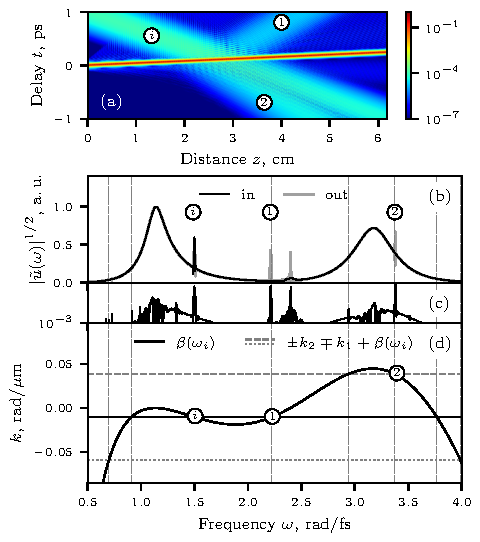
\includegraphics{{Figures/Fig3}.pdf}
  \caption{(color online) Scattering of a weak DW with carrier frequency $\omega_{\text{inc}} = 1.500$ on a soliton with first-component carrier frequency $\omega_{1} = 1.150$. (a) time-domain view (b) input and output spectra (c) resonance conditions diagram.}%
  \label{fig:Fig3}
\end{figure}

The third configuration (seen in Fig.~\ref{fig:Fig4}) is, in a sense, symmetric to the previous case. In here, again, the difference between $k_{1}$ and $k_{2}$ is significant and equation~\eqref{eq:Type1ResonanceCondition} is far from being degenerate, but in this case the resonances from the lower (i.e. ``$+, -$'') branch of~\eqref{eq:Type1ResonanceCondition} play a significant role. This is achieved by choosing the incident frequency greater than the carrier frequency of the second soliton component and enhanced by using an asymmetric seed soliton with $T_{1} = 30$~fs and $T_{2} = 10$~fs. This creates a solitray wave with the ampltiude of the second component almost equal to the ampltiude of the first component.

\begin{figure}[t]
  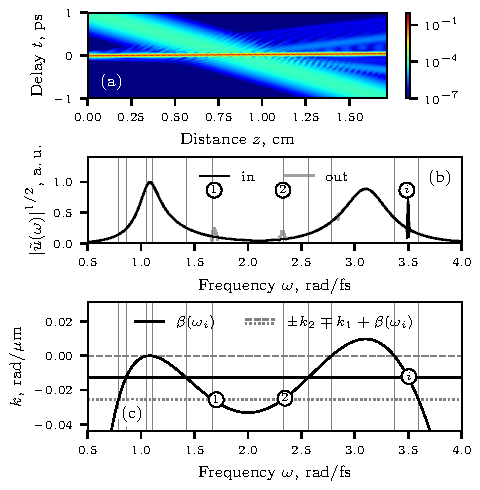
\includegraphics{{Figures/Fig4}.pdf}
  \caption{(color online) Scattering of a weak DW with carrier frequency $\omega_{\text{inc}} = 3.500$ on a soliton with first-component carrier frequency $\omega_{1} = 1.085$. (a) time-domain view (b) input and output spectra (c) resonance conditions diagram.}%
  \label{fig:Fig4}
\end{figure}

Overall, in all our experiments, we have only seen the scattered components corresponding to equations~\eqref{eq:Type0ResonanceCondition} and~\eqref{eq:Type1ResonanceCondition} and have never seen the components predicted~\eqref{eq:Type2ResonanceCondition} and~\eqref{eq:Type3ResonanceCondition}. In other words, the terms proportional to $\psi_{inc}^{*}$ in the right hand's side of equation~\eqref{eq:ScatteredFieldEquation} do not contribute significantly to the scattered radiation.

\section{Nonlinear effects}

When deriving the resonance conditions for scattering processes~\eqref{eq:Type0ResonanceCondition}~--~\eqref{eq:Type3ResonanceCondition} we assumed that the parameters of the solitons stay constant throughout propagation and scattering processes. This can be considered a reasonable approximation when the ampltiude of the incident wave stays negligible compared to the ampltidues of the individual soliton components. However, in the general case of a more intensive incident radiation this approximation breaks down. In this section we will briefly discuss two specific examples, where during scattering the interaction with the incident dispersive wave changes the parameters of the soliton. General setup of the experiments stay the same --- we consider scattering of a Gaussian pulse on an isolated two-color soliton --- but this time we pick DW ampltiude to be equal to 5\% of the soliton's maximum amplitude. This change might seem subtle, but this is enough to enrich the scattering dynamics.

In the first example (displayed in Figure~\ref{fig:Fig6}) we consider scattering of a dispersive wave with the incident frequency $\omega_{i} = 2.100$ on a soliton with $\omega_{1} = 1.010$. We see that an intensive dispersive wave can pull the soliton during scattering. This effect has been demonstrated before for the classical bright solitons of nonlinear Schr\"odinger equation~\cite{demircan2011controlling, tartara2015soliton}. What is remarkable about this interaction in case of a two-color soliton is the fact that the soliton appears to be stable during this process. Granted, the frequency offset gained by the soliton during the scattering is not especially prominent (panel~\ref{fig:Fig6}b.2), but at the same time the amplitude difference in both the frequency components stays under 1\% (panel~\ref{fig:Fig5}b.1), so almost no power loss occurs.

\begin{figure}[t]
  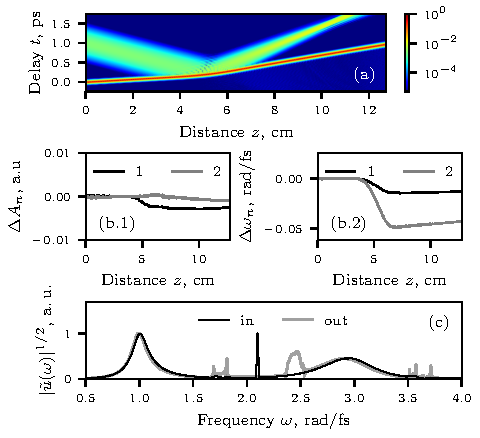
\includegraphics{{Figures/Fig6}.pdf}
  \caption{(color online) Scattering of an intensive DW with carrier frequency $\omega_{\text{inc}} = 2.100$ on a soliton with first-component carrier frequency $\omega_{1} = 1.010$. (a) time-domain view (b.1, 2) soliton amplitude and central frequency oscillations (c) output spectrum.}
  \label{fig:Fig6}
\end{figure}

In the second example (displayed in Figure~\ref{fig:Fig5}) we consider scattering of a dispersive wave with the incident frequency $\omega_{i} = 1.100$ on a soliton with $\omega_{1} = 1.010$. As it is evident from panels~\ref{fig:Fig5}b.1 and~\ref{fig:Fig5}b.2 the incident radiation pumps internal oscillations in the soliton during the scattering. The interaction of oscillating nonlinear waves, both the radiation and the scattering processes, is a well studied problem~\cite{driben2015resonant,oreshnikov2015interaction,wright2015ultrabroadband,conforti2015parametric,oreshnikov2017dispersive} and the common trait in this setting, independent on the nature of the soliton oscillations, is that the dispersive radiation produced (generated or scattered) by the soliton is polychromatic, i.e.\ it consists of several isolated spectral components. This is indeed what we see in output spectrum on panel~\ref{fig:Fig5}c. To explain this behavior let us return to equations~\eqref{eq:PerturbationEquation} and~\eqref{eq:ScatteredFieldEquation}. In the oscillating case the individual solitons $U_{1}$ and $U_{2}$ are no longer represented by a single spatial frequency $\propto e^{i k_{1} z}$ and $\propto e^{i k_{2} z}$, but instead each of them corresponds to a Fourier series
\begin{equation*}
  U_{n}(z, t) =
    \sum \limits_{N \in \mathbb{Z}}
    C_{n}(t) \exp \left(
      i k_{1} z + i \frac{2 \pi N}{Z_{0}} z
    \right),
\end{equation*}
where $Z_{0}$ is the oscillation period. This leads to a split in resonance conditions, and for the oscillating case equations \eqref{eq:CherenkovRadiationResonanceCondition}, \eqref{eq:FWMRadiationResonanceCondition}, \eqref{eq:Type0ResonanceCondition} and \eqref{eq:Type1ResonanceCondition} should read
\begin{gather}
  \label{eq:CherenkovRadiationresonanceConditionZ0}
  \tag{\ref{eq:CherenkovRadiationResonanceCondition}*}
  \beta(\omega) = k_{n}(\omega) + \frac{2 \pi N}{Z_{0}} \\
  \label{eq:FWMradiationResonanceConditionZ0}
  \tag{\ref{eq:FWMRadiationResonanceCondition}*}
  \beta(\omega) =
    2 k_{n}(\omega)  - k_{m}(\omega) +
    \frac{2 \pi N}{Z_{0}} \\
  \label{eq:Type0ResonanceConditionZ0}
  \tag{\ref{eq:Type0ResonanceCondition}*}
  \beta(\omega_{\text{sc}}) =
    \beta(\omega_{\text{inc}}) +
    \frac{2 \pi N}{Z_{0}} \\
  \label{eq:Type1ResonanceConditionZ0}
  \tag{\ref{eq:Type1ResonanceCondition}*}
  \beta(\omega_{\text{sc}}) =
    \pm k_{1} \mp k_{2} +
    \beta(\omega_{\text{inc}}) +
    \frac{2 \pi N}{Z_{0}},
\end{gather}
here $N \in \mathbb{Z}$ selects the harmonic.

The resonance conditions for the scattering process in the last simulation displayed on panel~\ref{fig:Fig5}d. In this process only the last two equations~\eqref{eq:Type0ResonanceCondition} and~\eqref{eq:Type1ResonanceCondition} are relevant. The solid black lines correspond to equation~\eqref{eq:Type0ResonanceCondition} with harmonics $N = -3, \dots, 0$. This harmonic split leads not only to the reflected part of the radiation \circled{1} becoming polychromatic, but also has the same effect on the incident component \circled{i}. Resonance condition~\eqref{eq:Type1ResonanceCondition} is represented by the gray dashed lines for harmonics $N = -3, \dots, +3$. It contributes to the scattered radiation twice: with a wide band \circled{2} that otherwise would degenerate into a sharp spectral line in a non-oscillating case, and with three wide spectral lines in vicinity of \circled{3} which is the contribution of the lower harmonics $N = -3, -2, -1$. One can notice that there is only two vertical lines corresponding to the numeric solution of~\eqref{eq:Type1ResonanceCondition} displayed around \circled{3}. This is merely due to a small numeric error in estimating the soliton wavenumber $k_{2}$ in the plotting procedure, which causes harmonic $N=-1$ to touch the dispersive rather than intersect it.

\begin{figure}[t]
  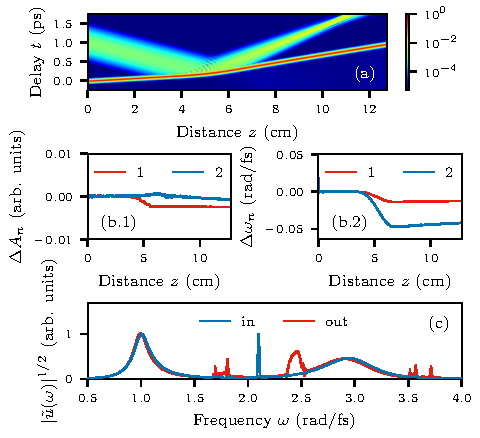
\includegraphics{{Figures/Fig5}.pdf}
  \caption{(color online) Scattering of an intensive DW with carrier frequency  $\omega_{\text{inc}} = 1.100$ on a soliton with first-component carrier frequency $\omega_{1} = 1.010$. (a) time-domain view (b.1, 2) soliton amplitude and central frequency oscillations (c) output spectrum (d) resonance condition diagram.}%
  \label{fig:Fig5}
\end{figure}

\section{Conclusion}

{
  % This is just a dummy text to see whether the general layout of the paper makes sense.
  \it
Pellentesque dapibus suscipit ligula.  Donec posuere augue in quam.  Etiam vel tortor sodales tellus ultricies commodo.  Suspendisse potenti.  Aenean in sem ac leo mollis blandit.  Donec neque quam, dignissim in, mollis nec, sagittis eu, wisi.  Phasellus lacus.  Etiam laoreet quam sed arcu.  Phasellus at dui in ligula mollis ultricies.  Integer placerat tristique nisl.  Praesent augue.  Fusce commodo.  Vestibulum convallis, lorem a tempus semper, dui dui euismod elit, vitae placerat urna tortor vitae lacus.  Nullam libero mauris, consequat quis, varius et, dictum id, arcu.  Mauris mollis tincidunt felis.  Aliquam feugiat tellus ut neque.  Nulla facilisis, risus a rhoncus fermentum, tellus tellus lacinia purus, et dictum nunc justo sit amet elit.

Aliquam erat volutpat.  Nunc eleifend leo vitae magna.  In id erat non orci commodo lobortis.  Proin neque massa, cursus ut, gravida ut, lobortis eget, lacus.  Sed diam.  Praesent fermentum tempor tellus.  Nullam tempus.  Mauris ac felis vel velit tristique imperdiet.  Donec at pede.  Etiam vel neque nec dui dignissim bibendum.  Vivamus id enim.  Phasellus neque orci, porta a, aliquet quis, semper a, massa.  Phasellus purus.  Pellentesque tristique imperdiet tortor.  Nam euismod tellus id erat.
}

\subsection{Acknowledgements}

\bibliographystyle{apsrev4-1}
\bibliography{Bibliography}

\end{document}

%%% Local Variables:
%%% mode: latex
%%% TeX-master: t
%%% End:
